% !TeX root = ../DistributedConsensus.tex
% !TeX spellcheck = en_GB
\chapter{Reducing Histories to Orders of Execution}\label{chap:order-of-execution}
	In this chapter, it is examined how it is possible to find an order of execution from a valid global history and it is shown that consensus can be reached on the found order of execution with an election.

\section{Order of Execution}
	A valid global history represents every action that has occurred on all the events of the workflow.
	It is desired to find an order of execution with excess information in the history removed without losing information regarding the order of the executions. To do this, we need to represent an execution as a single entity and furthermore find the minimum equivalent graph of the resulting order.
	
	\subsection{Single Entity Representing an Execution}
	In order to find a single representation of an execution, one approach could be to examine if a single action of an execution could describe all the relations to all the other executions. Doing this involves filtering all actions not chosen to be the representative of the execution, and since filtering nodes also removes their edges, happen before relations between executions would be lost. Therefore it is necessary to add a direct edge between representatives if there is already a path from one to the other in the history. Since the history is represented as a directed acyclic graph, the transitive closure of the graph provides the desired relations. Having found the transitive closure of the history, actions that are not the representative for an execution are removed from the graph along with their edge.
	
	Since every execution has actions of types \textit{Execute start} and \textit{Execute finish}, choosing one of these as the representative seems like a sensible choice. For any execution in a history, an action of type \textit{Execute start} always has a path to an action of type \textit{Execute finish}. Therefore the transitive property of directed acyclic graphs, states that in an execution the reachability of an action of type \textit{Execute start} is a superset of the reachability of the action of type \textit{Execute finish}, and therefore it contains more information about happens before relations. To conclude, actions of type \textit{Execute start} are the most sensible choice of these two types.
	
	\newpar We now extend the legend from \autoref{fig:representing:legend} with the following illustration types:
    
    \begin{figure}[H]
		\centering
		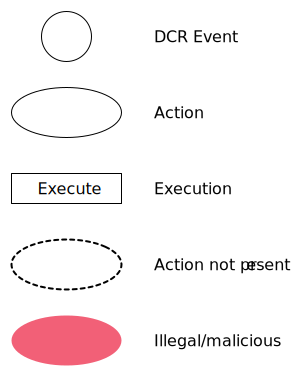
\includegraphics[height=0.25\textheight]{6validation/images/legend-extended.pdf}
		\caption{A legend showing what the different figures mean in the following sections.}
		\label{fig:representing:legend-extended}
	\end{figure}
	
	A situation where actions of type \textit{Execute start} is chosen as representatives is shown in \autoref{fig:problem:trans}. What becomes apparent in this figure, is that the first execution of event $A$ must happen before the first execution of event $B$. This is because two events that have a happen before relation must have any kind of relation in the workflow. If the events have a relation in the workflow, then they must execute serially equivalent. This ensures that an execution of one of the events must happen either before, or after an execution of the other. Therefore another approach must be taken.
	
	\newpar In \cite{sedgewick2011algorithms}, Sedgewick et. al. describes an implementation of transitive closure, which has a time complexity of $\mathcal{O}(V * (V + E))$ where V is the number of nodes and E is the number of edges in the graph.
	
	\begin{figure}
		\centering
		\includegraphics[width=\textwidth]{5orderofexecution/images/trans.pdf}
		\caption{The result of finding the transitive closure on from the actions of an event. Note that the topmost executions happen concurrently. So do the two lower executions.}
		\label{fig:problem:trans}
	\end{figure}
	
	\subsection{Collapsing}
	As described above, transitive closures are not an ideal way of representing an execution as a single entity and therefore collapsing is introduced.
	
	\newpar In \autoref{def:execution} an execution is defined to be all the actions representing the effects of the execution, as well as two actions with types \textit{Execute start} and \textit{Execute finish}. Even though incoming actions are stored on other events than the ones performing the executions, these actions are still initiated by the executing event and are therefore seen as being part of the execution. Since an event is only affected by the effects of other events or itself executing, any action is always part of \textit{some} execution of \textit{some} event, and therefore no action can happen outside an execution.

	\newpar In a global history, given an action of type \textit{Execute start}, the set of actions representing a single execution is found by taking each consecutive action with the same event ID until an action of type \textit{Execute finish} is found. Furthermore the incoming actions corresponding to the outgoing actions already found in the execution are added to the set.
	
	\newpar In \autoref{inv:historyinvariant} it is said that if a single action in one execution happens before another action in another execution, then no action from the second execution can happen before an action in the first. In other words this means, if there exists an action in execution $A$, that happens before an action in execution $B$, then $A$ happens before $B$, and $B$ cannot happen before $A$. Note that this does not mean that all actions in $A$ happens before all actions in $B$, which means some of the actions are in fact concurrent. This creates the need for an argument that $A$ \textit{does} happen before $B$ despite that some actions are concurrent.
	
	\newpar As stated in the previous section, because of serial equivalence, two events, where one has a relation to the other, can only execute in a way such that the result is the same as if one had executed before the other. Therefore any happens before relation any action in an execution has with any action outside of that execution actually applies to all actions in the execution. When this is the case, every action inside an execution is equal in terms of happens-before relations and therefore we can \textit{collapse} the execution into one single entity.
	
	\newpar An example of collapsing actions into executions is shown in \autoref{fig:orderofexecution:collapse}. This is the same example as used when describing transitive closure. Contrary to \autoref{fig:problem:trans}, the first execution of $A$ happens before the first execution of $B$.
	
	\begin{figure}[H]
		\centering
		\includegraphics[width=\textwidth]{5orderofexecution/images/collapse.pdf}
		\caption{The result of finding an execution using \textit{Collapse}. Note that some executions that previously were concurrent (\autoref{fig:problem:trans}) are now ordered.}
		\label{fig:orderofexecution:collapse}
	\end{figure}
	
	\newpar The collapsing algorithm can be be seen in \autoref{alg:collapse}. The algorithm gathers all actions of an execution and, after the single entity execution is created, creates all happens-before relations. In order to do so, it uses a few helper functions. \texttt{GetEdgesToOtherExecutions} together with \texttt{MapOldEdgesToNewIDs} represent the translation of edges of actions in one execution to actions in another execution, to edges from execution entity to execution entity.
	
	\begin{algorithm}[H]
		\begin{algorithmic}
			\Function{Collapse}{history} \textbf{returns} an order of execution \State
			actionMapper $\leftarrow$ \Call{EmptyMap}{ }
			\State executeStartActions $\leftarrow$ \Call{FilterByType}{ExecuteStart, history}
			\State
			\ForAll{action \textbf{in} executeStartActions}
				\Comment Loop 1
				\State execution $\leftarrow$ \Call{FindSingleExecution}{action}
				\State uniqueId $\leftarrow$ \Call{GenerateUniqueId}{ }
				\ForAll{executionAction \textbf{in} execution}\State
					actionMapper $\leftarrow$ \Call{Add}{action.Id, uniqueId, actionMapper} 
				\EndFor
			\EndFor
			\State
			\State orderOfExecution $\leftarrow$ \Call{EmptyGraph}{ }
			\State
			\ForAll{oldActionID, newActionID \textbf{in} actionMapper}
				\Comment Loop 2
				\State oldEdges $\leftarrow$ \Call{GetEdgesToOtherExecutions}{oldActionId, history}
				\State edges $\leftarrow$ \Call{MapOldEdgesToNewIDs}{oldEdges, actionMapper}
				\State newAction $\leftarrow$ \Call{CreateAction}{newActionId, edges}
			\State
			orderOfExecution $\leftarrow$ \Call{AddNode}{newAction, orderOfExecution} \State\Comment{This requires \Call{AddNode}{} to merge edge sets when existing nodes are added}
			\EndFor\State
			\Return orderOfExecution
			\EndFunction
		\end{algorithmic}
		\caption{Collapse algorithm}
		\label{alg:collapse}
	\end{algorithm}
	
	\noindent One of the properties the collapsed order of execution has, is that, for two executions to be concurrent the executing events must be independent, as described in \cite{debois2015concurrency}, however, not all independent\- events create concurrent executions.
	
	All non-independent events cannot execute concurrently, and to demonstrate this, we will show that if any of the properties of independent events are not present between a pair of events, therefore making them non-independent, then collapse will order the executions.
	
	\begin{enumerate}
		\item \textit{No event included by $E$ is excluded by $F$ and vice versa}: This property is violated if $E$ includes an event, $G$ that $F$ excludes. The incoming actions on $G$ will allow collapse to order the executions of $E$ and $F$.
		\item \textit{$E$ requires a response from some $G$ iff $F$ does}: This property is violated if $E$ has a response relation to $F$, but $F$ does not have a response relation to itself. In this case, an execution of $E$ results in incoming actions on $F$. Any execution of $F$ is always before or after these incoming actions.
		\item \textit{Neither event is a condition for the other}: This property is violated if $E$ is a condition for $F$. In this case the incoming actions from the execution of $F$ on $E$, enables the ordering of executions of the events.
		\item \textit{Neither event includes or excludes the other}: This property is violated if $E$ includes $F$. In this case the incoming actions from the execution of $E$ on $F$, enables the ordering of executions of the events.
		\item \textit{Neither event includes or excludes a condition of the other}: This property is violated if $E$ excludes $G$ which is a condition of $F$. Recall that conditions in the implementation are checked by the executing event. This means that any execution of $F$ will result in incoming actions on $G$. Also the execution of $E$ will result in incoming actions on $G$. Therefore the incoming actions on $G$ will allow collapse to order the executions of $E$ and $F$.
	\end{enumerate}
	
	To argue that the collapse algorithm correctly describes the relations between executions \autoref{inv:historyinvariant} is examined. The invariant states that if there exist any action in execution $A$ with a relation to execution $B$, then it must not be true the other way around. Therefore for collapse to be correct every single execution entity must have the abide to the invariant. 
	
	Since the set of relations the entity representing an execution has to other executions is the union of the sets of all the relations the actions of the execution had to other executions, then the set cannot contain relations which violates the invariant, because then the invariant would already be violated before collapsing. If the invariant is violated in the union set, then there must have been an action in an execution $A$ that happens before an action in an execution $B$ and an action in $B$ that happens before an action in $A$ in the original collection of sets representing the executions.
	
	\newpar The algorithm runs in a time complexity of $\mathcal{O}(N+E)$ where $N$ is the number of actions and $E$ is the number of edges in the history. This is due to \texttt{FindSingleExecution} and \texttt{executeStartActions} are inversely proportional and together constitutes the amount of actions in the graph. Therefore the overall complexity of \texttt{loop 1} is linear to the amount of actions. \texttt{Loop 2} iterates over every action in the history, furthermore every edge in the history is iterated over since they are retrieved for every action with \texttt{GetEdgesToOTherExecutions}. \texttt{MapOldEdgesToNewIds}, \texttt{CreateAction} runs in constant time and \texttt{AddNode} runs linear time to the amount of edges between executions, then the first part of the second loop is the dominant factor. Therefore the second loop run in $\mathcal{O}(N+E)$, and is then the most dominant factor of the entire algorithm.
	
	\subsection{Transitive Reduction}
	Redundant edges might still exist in between executions after collapsing a history. An edge is redundant in cases where there exists a non-direct path from an execution to another execution, but there also exists a direct edge between the two executions. In this case the direct edge is redundant and can be removed, since it does not contribute extra information in regards to the ordering of the executions, as it only explicitly expresses what is implicitly available. Removing the direct edge will not affect the ordering or reachability of the order of execution, but rather simplify it.
	
	\newpar Figure \ref{fig:orderofexecution:collapsing} illustrates a case where a redundant edge exists between executions of event $B$ and $A$, since there is a path from the execution of event $B$ to the execution of $A$ through the execution of event $C$. Recall that the order of execution is represented as a directed acyclic graph and that it is possible to find a minimal equivalent graph for such a graph.
	
	\begin{figure}[H]
		\centering
		\includegraphics[width=\textwidth]{5orderofexecution/images/transitive-example-collapse.pdf}
		\caption{The result of collapsing actions in the histories of three events.}
		\label{fig:orderofexecution:collapsing}
	\end{figure}
	
	\newpar In directed acyclic graphs the transitive reduction produces the minimal equivalent graph. A naive algorithm for finding the transitive reduction on an order of execution is shown in \autoref{alg:orderofexecution:reduction}.
	
	\begin{algorithm}[H]
		\begin{algorithmic}
			\Function{Transitive-Reduction}{$orderOfExecution$}
				\ForAll{$execution1$ \textbf{in} $orderOfExecution$}
				\Comment Loop 1
					\ForAll{$execution2$ \textbf{in} $orderOfExecution$}
					\Comment Loop 2
						\If{\Call{PathExists}{$execution1$, $execution2$, $orderOfExecution$}}
							\ForAll{$execution3$ \textbf{in} $execution2.edges$}
							\Comment Loop 3
								\If{\Call{EdgeExists}{$execution1$, $execution3$}}
									\State $orderOfExecution$ $\leftarrow$ \State \hspace{2em}\Call{RemoveEdge} {$execution1$, $execution3$, $orderOfExecution$}
								\EndIf
							\EndFor
						\EndIf
					\EndFor
				\EndFor
			\State
			\Return $orderOfExecution$
			\EndFunction
		\end{algorithmic}
		\caption{Transitive Reduction Algorithm}
		\label{alg:orderofexecution:reduction}
	\end{algorithm}
	
	\newpar The shown algorithm for transitive reduction has a time complexity of $\mathcal{O}(n^2(n+e))$ where $n$ is the number of executions and $e$ is the number of happens-before relations between executions. Since \texttt{EdgeExists} and \texttt{RemoveEdge} run in constant time, \texttt{loop 3} has a time complexity of $\mathcal{O}(E)$ because in worst case \texttt{loop 2} iterates over all executions in the graph and \texttt{execution2.edges} represents all edges in the graph. \texttt{PathExists} has a time complexity of $\mathcal{O}(N+E)$ because each node is visited over each edge. Therefore \texttt{PathExists} becomes the dominant factor of the second loop. \texttt{Loop 1} and \text{Loop 2} has a time complexity of $\mathcal{O}(N^2)$ and therefore the combined time complexity of the entire algorithm is $\mathcal{O}(n^2(n+e))$.
	
	\begin{figure}[H]
		\centering
		\includegraphics[height=0.35\textheight]{5orderofexecution/images/reduce-before-after.pdf}
		\caption{The result of reducing an order of execution with redundant edges.}
		\label{fig:orderofexecution:reduce-before-after}
	\end{figure}

	\noindent As with the input to the merge algorithm presented in \autoref{chap:connecting-histories}, the input of the collapse algorithm must be a valid global history for the algorithm to produce a valid order of execution. If the global history is not valid, then the validity of the order of execution cannot be guaranteed. As the transitive reduction algorithm only remove redundant information from an order of execution, the same problem arises.
	
	We will see in \autoref{chap:validation} that an order of execution can be used to validate certain kinds of cheating.

	\section{Election}
	Assuming that the found order of execution is valid, we want to know if the processes hosting the events of the workflow can reach consensus on this order of execution.
	
	Recall the three requirements for a consensus algorithm: Termination, agreement, and integrity. We want to make an election that fulfils these requirements.
	
	\newpar For this consensus problem, the proposed value is the global order of execution and for a process hosting an event to accept a proposed global order of execution, it must be able to map all the actions of its local history onto the executions in the global order of execution.
	
	\newpar To map actions in the local history to an order of execution the following procedure is followed:

	\begin{itemize}
		\item If an action has the type \textit{Execute start}, then all consecutive actions until an action of type \textit{Execute finish} is found are part of the same execution of the event itself.
		\item If an incoming action is found, then all following actions with the same counterpart ID but distinct action types represent an execution of the counterpart event.
		\begin{itemize}
			\item This implies that if a new action with the same counterpart ID and an action type not distinct from the ones before it, it must represent the beginning of a new execution of the counterpart event.
			\item It also implies that if an incoming action with another counterpart ID is found, then this is the beginning of an execution of the event with the new counterpart ID.
		\end{itemize}
	\end{itemize}
	
	\noindent Because the mapping is created consecutively and because the local history is in total order, the mapped executions must have the same happens before relations as the order in which they are found. Furthermore, if an execution of an event exists in the mapping of the local history, then all executions of that event must be represented in the local history. Therefore the first mapping of an execution in the local history must be the execution of the specified event that  happens before any other execution of that event in the global history.
	
	An example of mapping actions of local histories to executions are shown in \autoref{fig:orderofexecution:localmapping}. In the figure it is seen that pairs of actions with types \textit{Execute start} and \textit{Execute finish} represent executions of the local event. Furthermore, because event $A$ included event $B$ twice, two executions of $A$ must have happened. Also note that the order of the actions are preserved in the local order of execution.
	
	\begin{figure}[H]
		\centering
		\includegraphics[width=.4\textwidth]{5orderofexecution/images/election-mapping.pdf}
		\caption{An example of mapping actions of local histories to executions}
		\label{fig:orderofexecution:localmapping}
	\end{figure}
	
	\newpar From any mapping of an execution found in the global order of execution it should be possible to find the next mapping of an execution only by traversing edges in the global order of execution.
	
	If the local history matches the global order of execution, then the process hosting the event accepts the proposed value.
	
	\newpar We have now described how a proposed value can be voted on. It still needs to be discussed how an election is initiated.
	
	\newpar As described in \autoref{chap:connecting-histories}, the client retrieves all local histories of a workflow, then it merges, collapses, and reduces the histories into an global order of execution. Therefore the client is the only process able to propose a value that all processes hosting events can reach consensus on. Because the client already knows all events in order to retrieve their histories, it can propose the global order of execution to each of them and await their answers.
	
	\newpar If the local histories are valid, and all of the presented algorithms are correct, then all processes hosting events will reach consensus on the proposed global order of execution, because the local orders of execution are preserved in the global. Therefore both the agreement and integrity requirement of the election is fulfilled. Because we do not allow processes to crash while carrying out a task, every process must at some point respond to the proposal thereby setting its decided value. Therefore the termination requirements is fulfilled.
	
	\newpar If any process does not vote in favour of the order of execution it implies that either a local history was invalid, the proposer created an incorrect order of execution, or the process incorrectly voted against the proposed value. In either of the cases, a malicious process must exist in the system, and therefore if no process votes against the proposed value, we have solved the problem of reaching consensus on an order of execution of an execution of a distributed DCR graph when no malicious processes are present in the system.